\section{Implementation}

%----------------------------------------------------------
\subsection{Feature Engineering via Grouped PCA}
%----------------------------------------------------------

\subsubsection{Motivation}

The raw training dataset contains 246 meteorological predictors, many of which exhibit extreme multi-collinearity. For instance, ensemble forecasts from the NMME model and geopotential height fields (\texttt{hgt}) at various atmospheric levels often contain near-identical variance patterns across their respective columns. Feeding these 246 raw features directly into a regression model risks overfitting and unnecessary computational overhead. We implement a \textbf{Grouped PCA} strategy to compress these blocks independently, ensuring that we capture the dominant physical signals while discarding redundant noise.

\subsubsection{Dynamic Variance-Based PCA}

Unlike standard PCA which uses a fixed number of components $k$, we employ a dynamic thresholding approach. For each meteorological group $g$, we retain the minimum number of components $k_g$ such that the cumulative explained variance ratio $C(k_g)$ meets a predefined threshold $\eta = 0.95$:

\begin{equation}
    k_g = \min \left\{ k : \sum_{j=1}^{k} \lambda_j / \sum_{i=1}^{p_g} \lambda_i \ge \eta \right\}
    \label{eq:dynamic_pca}
\end{equation}

where $\lambda_j$ are the eigenvalues of the group's covariance matrix ordered descendingly, and $p_g$ is the original number of features in group $g$. This ensures that while the dimensionality is reduced, 95\% of the information (variance) within each physical domain is preserved.

\subsubsection{Grouped PCA Design and Results}

We partition the feature space into 11 specialized groups based on their physical variables. Features not categorized into these groups (e.g., temporal indices or specific local coordinates) are preserved in their original form. As shown in Table~\ref{tab:pca_results}, this grouping strategy reduces the total feature count from 246 to 92.

\begin{table}[htbp]
  \centering
  \caption{Grouped PCA Results ($\eta = 0.95$ threshold).}
  \label{tab:pca_results}
  \begin{tabular}{lccc}
    \toprule
    Group Name & Input Cols & Output PCs & Expl. Variance \\
    \midrule
    \texttt{nmme\_tmp34w} & 20  & 2  & 97.2\% \\
    \texttt{nmme\_tmp56w} & 10  & 1  & 97.4\% \\
    \texttt{nmme\_prate}  & 40  & 12 & 95.3\% \\
    \texttt{hgt10}        & 10  & 2  & 97.0\% \\
    \texttt{hgt100}       & 10  & 2  & 95.8\% \\
    \texttt{hgt500}       & 10  & 6  & 96.0\% \\
    \texttt{hgt850}       & 10  & 8  & 96.9\% \\
    \texttt{sst}          & 10  & 2  & 96.3\% \\
    \texttt{icec}         & 10  & 3  & 96.6\% \\
    \texttt{wind\_uv}      & 80  & 21 & 95.4\% \\
    \texttt{tele}         & 5   & 2  & 99.1\% \\
    \midrule
    \textbf{Total / Summary} & \textbf{215} & \textbf{61} & \textbf{95\% Avg.} \\
    \bottomrule
  \end{tabular}
\end{table}

The final feature set consists of 61 principal components and 31 original features, resulting in a total of 92 predictors. This transformation effectively reduces the feature space by approximately 62\% while maintaining high physical fidelity. The PCA mapping is fitted only on the training set to prevent data leakage.

%----------------------------------------------------------
\subsection{Predictive Models}
%----------------------------------------------------------

All candidate models ingest the same refined 92-dimensional feature set. To ensure robust convergence and treat the principal components and raw features on an equal footing, each model is wrapped in a \texttt{sklearn.pipeline.Pipeline}. 

The pipeline prepends a \texttt{StandardScaler} to the estimator, which normalizes the inputs to zero mean and unit variance. This step is critical for the numerical stability of both linear methods (satisfying Gaussian assumptions) and tree-based methods (ensuring consistent regularization effects).

\subsubsection{Lasso Regression}

Lasso augments the ordinary least-squares objective with an $\ell_1$ penalty:

\begin{equation}
  \hat{\boldsymbol{\beta}}_{\text{Lasso}} =
  \underset{\boldsymbol{\beta}}{\arg\min}\;
  \frac{1}{n}\|\mathbf{y} - \mathbf{X}\boldsymbol{\beta}\|_2^2
  + \alpha \|\boldsymbol{\beta}\|_1.
  \label{eq:lasso}
\end{equation}

The $\ell_1$ norm induces sparsity by driving irrelevant coefficients exactly
to zero, effectively performing automatic feature selection.

\subsubsection{Elastic Net}

Elastic Net combines the $\ell_1$ and $\ell_2$ penalties,
balancing sparsity and grouping effects:

\begin{equation}
  \hat{\boldsymbol{\beta}}_{\text{EN}} =
  \underset{\boldsymbol{\beta}}{\arg\min}\;
  \frac{1}{n}\|\mathbf{y} - \mathbf{X}\boldsymbol{\beta}\|_2^2
  + \alpha\!\left[\rho\|\boldsymbol{\beta}\|_1
    + \frac{1-\rho}{2}\|\boldsymbol{\beta}\|_2^2\right],
  \label{eq:elasticnet}
\end{equation}

where $\rho \in [0,1]$ is the $\ell_1$ mixing ratio (\texttt{l1\_ratio}).

\subsubsection{Random Forest}

Random Forest constructs an ensemble of $B$ decision trees
$\{T_b\}_{b=1}^B$, each grown on a bootstrap replicate of the training data
and using a random subset of $\lfloor\sqrt{p}\rfloor$ features at every split
(CART criterion for regression):

\begin{equation}
  \hat{y} = \frac{1}{B}\sum_{b=1}^{B} T_b(\mathbf{x}).
  \label{eq:rf}
\end{equation}

The randomisation over both samples and features decorrelates the trees,
reducing variance without substantially increasing bias.

\subsubsection{XGBoost}

XGBoost (eXtreme Gradient Boosting) builds an additive ensemble
of regression trees in a stage-wise fashion by minimising a regularised
second-order Taylor expansion of the loss:

\begin{equation}
  \mathcal{L}^{(t)} = \sum_{i=1}^{n}
  \left[g_i f_t(\mathbf{x}_i) + \tfrac{1}{2}h_i f_t^2(\mathbf{x}_i)\right]
  + \Omega(f_t),
  \label{eq:xgboost}
\end{equation}

where $g_i = \partial_{\hat{y}^{(t-1)}}\ell(y_i, \hat{y}^{(t-1)})$ and
$h_i = \partial^2_{\hat{y}^{(t-1)}}\ell(y_i, \hat{y}^{(t-1)})$ are the first
and second gradients of the MSE loss, and
$\Omega(f_t) = \gamma T + \tfrac{1}{2}\lambda\|\mathbf{w}\|^2$ penalises tree
complexity ($T$: leaf count, $\mathbf{w}$: leaf weights).

\subsubsection{LightGBM}

LightGBM shares the GBDT framework of XGBoost but introduces two key
algorithmic innovations for scalability.
\textit{Gradient-based One-Side Sampling} (GOSS) retains all instances
with large gradients $|g_i| > \theta$ while randomly sub-sampling those
with small gradients at ratio $\beta$, yielding an unbiased variance
estimate with fewer data points:

\begin{equation}
  \tilde{\mathcal{G}}_j = \sum_{i \in A} g_i
    + \frac{1-\beta}{\beta} \sum_{i \in B} g_i,
  \label{eq:goss}
\end{equation}

where $A$ is the set of top-$a$ large-gradient instances and $B$ is a random
sample of size $b$ from the remainder.
\textit{Exclusive Feature Bundling} (EFB) further merges mutually exclusive
sparse features to reduce the effective feature dimension.
LightGBM grows trees \emph{leaf-wise} rather than level-wise,
selecting the leaf with the maximum gain $\Delta\mathcal{L}$ at each step,
enabling deeper effective trees with fewer splits.

\subsubsection{CatBoost}

CatBoost introduces \textit{Ordered Boosting} to
eliminate the target leakage inherent in standard GBDT.
For each training example $i$, the residual is computed using a model
$M_{\sigma(i)}$ trained only on examples preceding $i$ in a random
permutation $\sigma$:

\begin{equation}
  r_i = y_i - M_{\sigma(i)}(\mathbf{x}_i),
  \quad \text{where } M_{\sigma(i)} \text{ is fitted on }
  \{(\mathbf{x}_j, y_j) : \sigma(j) < \sigma(i)\}.
  \label{eq:catboost}
\end{equation}

This ordered scheme ensures that each gradient estimate is unbiased
with respect to the target, preventing the subtle overfitting that affects
classical GBDT implementations.
CatBoost also implements an efficient ordered target statistics encoding
for categorical variables.

%----------------------------------------------------------
\subsection{Weighted Blending Ensemble}
%----------------------------------------------------------

Rather than using a complex stacking approach with out-of-fold predictions,
we employ a simpler and more robust \textbf{weighted blending} strategy
that combines the best tree-based model (CatBoost) with the best linear model
(Elastic Net). The rationale is that tree-based and linear models capture
fundamentally different patterns in the data: tree models excel at modelling
non-linear interactions, while linear models capture global trends and are
less prone to overfitting. This diversity is key to effective ensembling.

The blending prediction is defined as:

\begin{equation}
  \hat{y}_{\text{blend}} = \alpha \cdot \hat{y}_{\text{CatBoost}}
    + (1 - \alpha) \cdot \hat{y}_{\text{ElasticNet}},
  \label{eq:blending}
\end{equation}

where $\alpha \in [0, 1]$ is the blending weight. We search for the optimal
$\alpha$ by evaluating the RMSE on the 20\% held-out validation set over
a fine grid $\alpha \in \{0.00, 0.01, 0.02, \ldots, 1.00\}$, selecting the
value that minimises the validation RMSE. This approach avoids the
computational cost of cross-validated stacking (which requires re-training
all base models multiple times) while still leveraging model diversity.

%==========================================================
%  Section 4: Evaluation
%==========================================================
\section{Evaluation}

%----------------------------------------------------------
\subsection{Evaluation Metrics}
%----------------------------------------------------------

Model performance is quantified with two complementary metrics.

\paragraph{Root Mean Squared Error (RMSE).}
\begin{equation}
  \text{RMSE} = \sqrt{\frac{1}{n}\sum_{i=1}^{n}(y_i - \hat{y}_i)^2}.
  \label{eq:rmse}
\end{equation}
RMSE is expressed in the same unit as the target variable
and penalises large errors more heavily than small ones.

\paragraph{Coefficient of Determination ($R^2$).}
\begin{equation}
  R^2 = 1 - \frac{\sum_{i=1}^{n}(y_i - \hat{y}_i)^2}
                  {\sum_{i=1}^{n}(y_i - \bar{y})^2},
  \label{eq:r2}
\end{equation}
where $\bar{y}$ is the mean of the observed values.
$R^2 = 1$ indicates a perfect fit; $R^2 = 0$ means the model performs
no better than predicting the mean.

%----------------------------------------------------------
\subsection{Experimental Results}
%----------------------------------------------------------

\subsubsection{Individual Model Performance}

Table~\ref{tab:model_results} reports the held-out test RMSE and $R^2$ for
all six models, evaluated on a temporal 80/20 split (training on the first
80\% of samples sorted by date, testing on the remaining 20\%).

\begin{table}[htbp]
  \centering
  \caption{Individual model performance (80/20 temporal split).}
  \label{tab:model_results}
  \begin{tabular}{lcc}
    \toprule
    Model         & Test RMSE & Test $R^2$ \\
    \midrule
    CatBoost      & \textbf{1.0959} & \textbf{0.9703} \\
    LightGBM      & 1.2001  & 0.9644 \\
    XGBoost       & 1.2466  & 0.9615 \\
    ElasticNet    & 1.5153  & 0.9432 \\
    Lasso         & 1.6224  & 0.9348 \\
    Random Forest & 1.7799  & 0.9216 \\
    \bottomrule
  \end{tabular}
\end{table}

The three gradient boosting methods (CatBoost, LightGBM, XGBoost) consistently
outperform the linear and Random Forest baselines on the test set.
CatBoost achieves the lowest test RMSE of \textbf{1.0959} with $R^2 = 0.9703$.

\subsubsection{Blending Ensemble Performance}

To explore whether combining a tree-based model with a linear model can
further improve predictions, we perform weighted blending between CatBoost
and Elastic Net on the 20\% validation set.

Figure~\ref{fig:alpha_search} shows the RMSE as a function of the blending
weight $\alpha$. The optimal weight is found at $\alpha = 0.78$, meaning
the final prediction is dominated by CatBoost (78\%) with a 22\% contribution
from Elastic Net.

\begin{figure}[htbp]
  \centering
  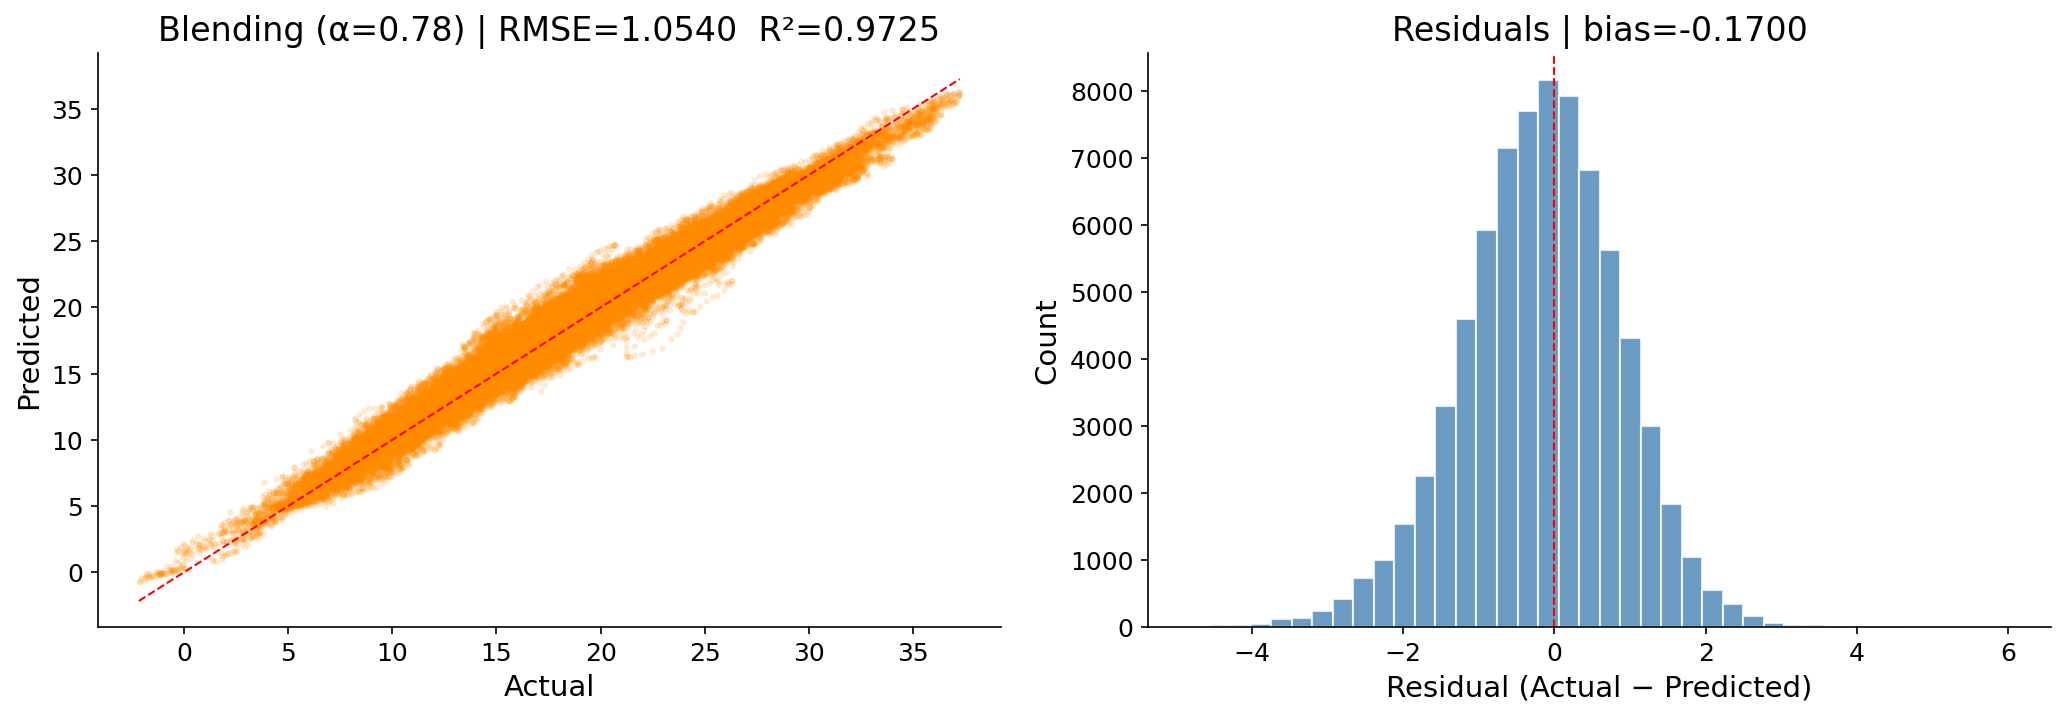
\includegraphics[width=0.85\textwidth]{../outputs/figures/ensemble_blending_20260407_201942.png}
  \caption{Blending weight search: validation RMSE vs.\ $\alpha$
    ($\hat{y} = \alpha \cdot \text{CatBoost} + (1-\alpha) \cdot \text{ElasticNet}$).
    The dashed red line marks the optimal $\alpha = 0.78$;
    the dotted grey line shows CatBoost-only performance.}
  \label{fig:alpha_search}
\end{figure}

Table~\ref{tab:ensemble_results} compares the blending result with the
individual base models.

\begin{table}[htbp]
  \centering
  \caption{Blending ensemble results (CatBoost + ElasticNet).}
  \label{tab:ensemble_results}
  \begin{tabular}{lccc}
    \toprule
    Method & Weight & Test RMSE & Test $R^2$ \\
    \midrule
    CatBoost (base)            & --    & 1.0959 & 0.9703 \\
    ElasticNet (base)          & --    & 1.5153 & 0.9432 \\
    \textbf{Blending} ($\alpha=0.78$) & 0.78 / 0.22 & \textbf{1.0540} & \textbf{0.9725} \\
    \bottomrule
  \end{tabular}
\end{table}

The blending ensemble achieves a test RMSE of \textbf{1.0540}, representing
a \textbf{3.82\%} improvement over CatBoost alone. This confirms that
combining a tree-based model with a linear model---which captures complementary
patterns in the data---yields a meaningful improvement, even when the linear
model is individually much weaker. The final $R^2$ of 0.9725 indicates that
the blended model explains over 97\% of the variance in the held-out test set.
